\documentclass[12pt,letterpaper]{article}

\usepackage[brazilian]{babel}
\usepackage[utf8]{inputenc}
\usepackage[T1]{fontenc}

\usepackage{fullpage}
\usepackage[top=2cm, bottom=4.5cm, left=2.5cm, right=2.5cm]{geometry}
\usepackage{amsmath,amsthm,amsfonts,amssymb,amscd}
\usepackage{lastpage}
\usepackage{enumerate}
\usepackage{fancyhdr}
\usepackage{mathrsfs}
\usepackage{xcolor}
\usepackage{graphicx}
\usepackage{listings}
\usepackage{hyperref}

\hypersetup{%
  colorlinks=true,
  linkcolor=blue,
  linkbordercolor={0 0 1}
}
 
\renewcommand\lstlistingname{Algorithm}
\renewcommand\lstlistlistingname{Algorithms}
\def\lstlistingautorefname{Alg.}

\lstdefinestyle{Python}{
    language        = Python,
    frame           = lines, 
    basicstyle      = \footnotesize,
    keywordstyle    = \color{blue},
    stringstyle     = \color{green},
    commentstyle    = \color{red}\ttfamily
}

\setlength{\parindent}{0.0in}
\setlength{\parskip}{0.05in}

% Edit these as appropriate
\newcommand\course{Rener Oliveira}
\newcommand\hwnumber{1}                  % <-- homework number
\newcommand\NetIDa{netid19823}           % <-- NetID of person #1
\newcommand\NetIDb{netid12038}           % <-- NetID of person #2 (Comment this line out for problem sets)

\pagestyle{fancyplain}
\headheight 35pt              % <-- Comment this line out for problem sets (make sure you are person #1)
\chead{\textbf{\Large Lista 1 \\ Curvas e Superfícies}}
\rhead{\small{\course \\ \today}}
\lfoot{}
\cfoot{}
\rfoot{\small\thepage}
\headsep 1.5em

\begin{document}
	
	\large{\textbf{Observação:}} Todos os arquivos Geogebra citados neste texto, estão disponíveis \href{https://gvmail-my.sharepoint.com/:f:/g/personal/b39398_fgv_edu_br/Euu4MOsNJNNEs3nZTImei1MBK16JRBHHiWUX9SxQeItAEg}{nesta pasta compartilhada do OneDrive}.
\begin{enumerate}
	\item Encontrar uma curva (parametrizada) $\alpha(t) : t \in I \to \mathbb{R}^2$; cujo traço seja o círculo
	$x^2 + y^2 = 1$; de maneira que $t$ percorra o círculo no sentido anti-horário e tenhamos $\alpha (0) = (0, 1)$. Faça o desenho em Geogebra, incluindo a animação do vetor tangente percorrendo a curva.
	\subitem \textbf{Solução:} Tome $\alpha (t) = (\cos t,\sin t)$. Veja que $\alpha(0)=(\cos 0,\sin 0) = (0,1)$. O vetor tangente é dado por $\vec v(t)=\alpha '(t)=(-\sin t,\cos t)$. Na Figura \ref{ex1}, vemos uma representação da animação desejada com $t=0.4$. Ao executar a animação (arquivo \href{https://gvmail-my.sharepoint.com/:f:/g/personal/b39398_fgv_edu_br/Euu4MOsNJNNEs3nZTImei1MBK16JRBHHiWUX9SxQeItAEg}{ex1.ggb}) percebe-se que de fato o sentido do movimento é anti-horário.
	\begin{figure}[!htb]
		\centering
		\label{ex1}
		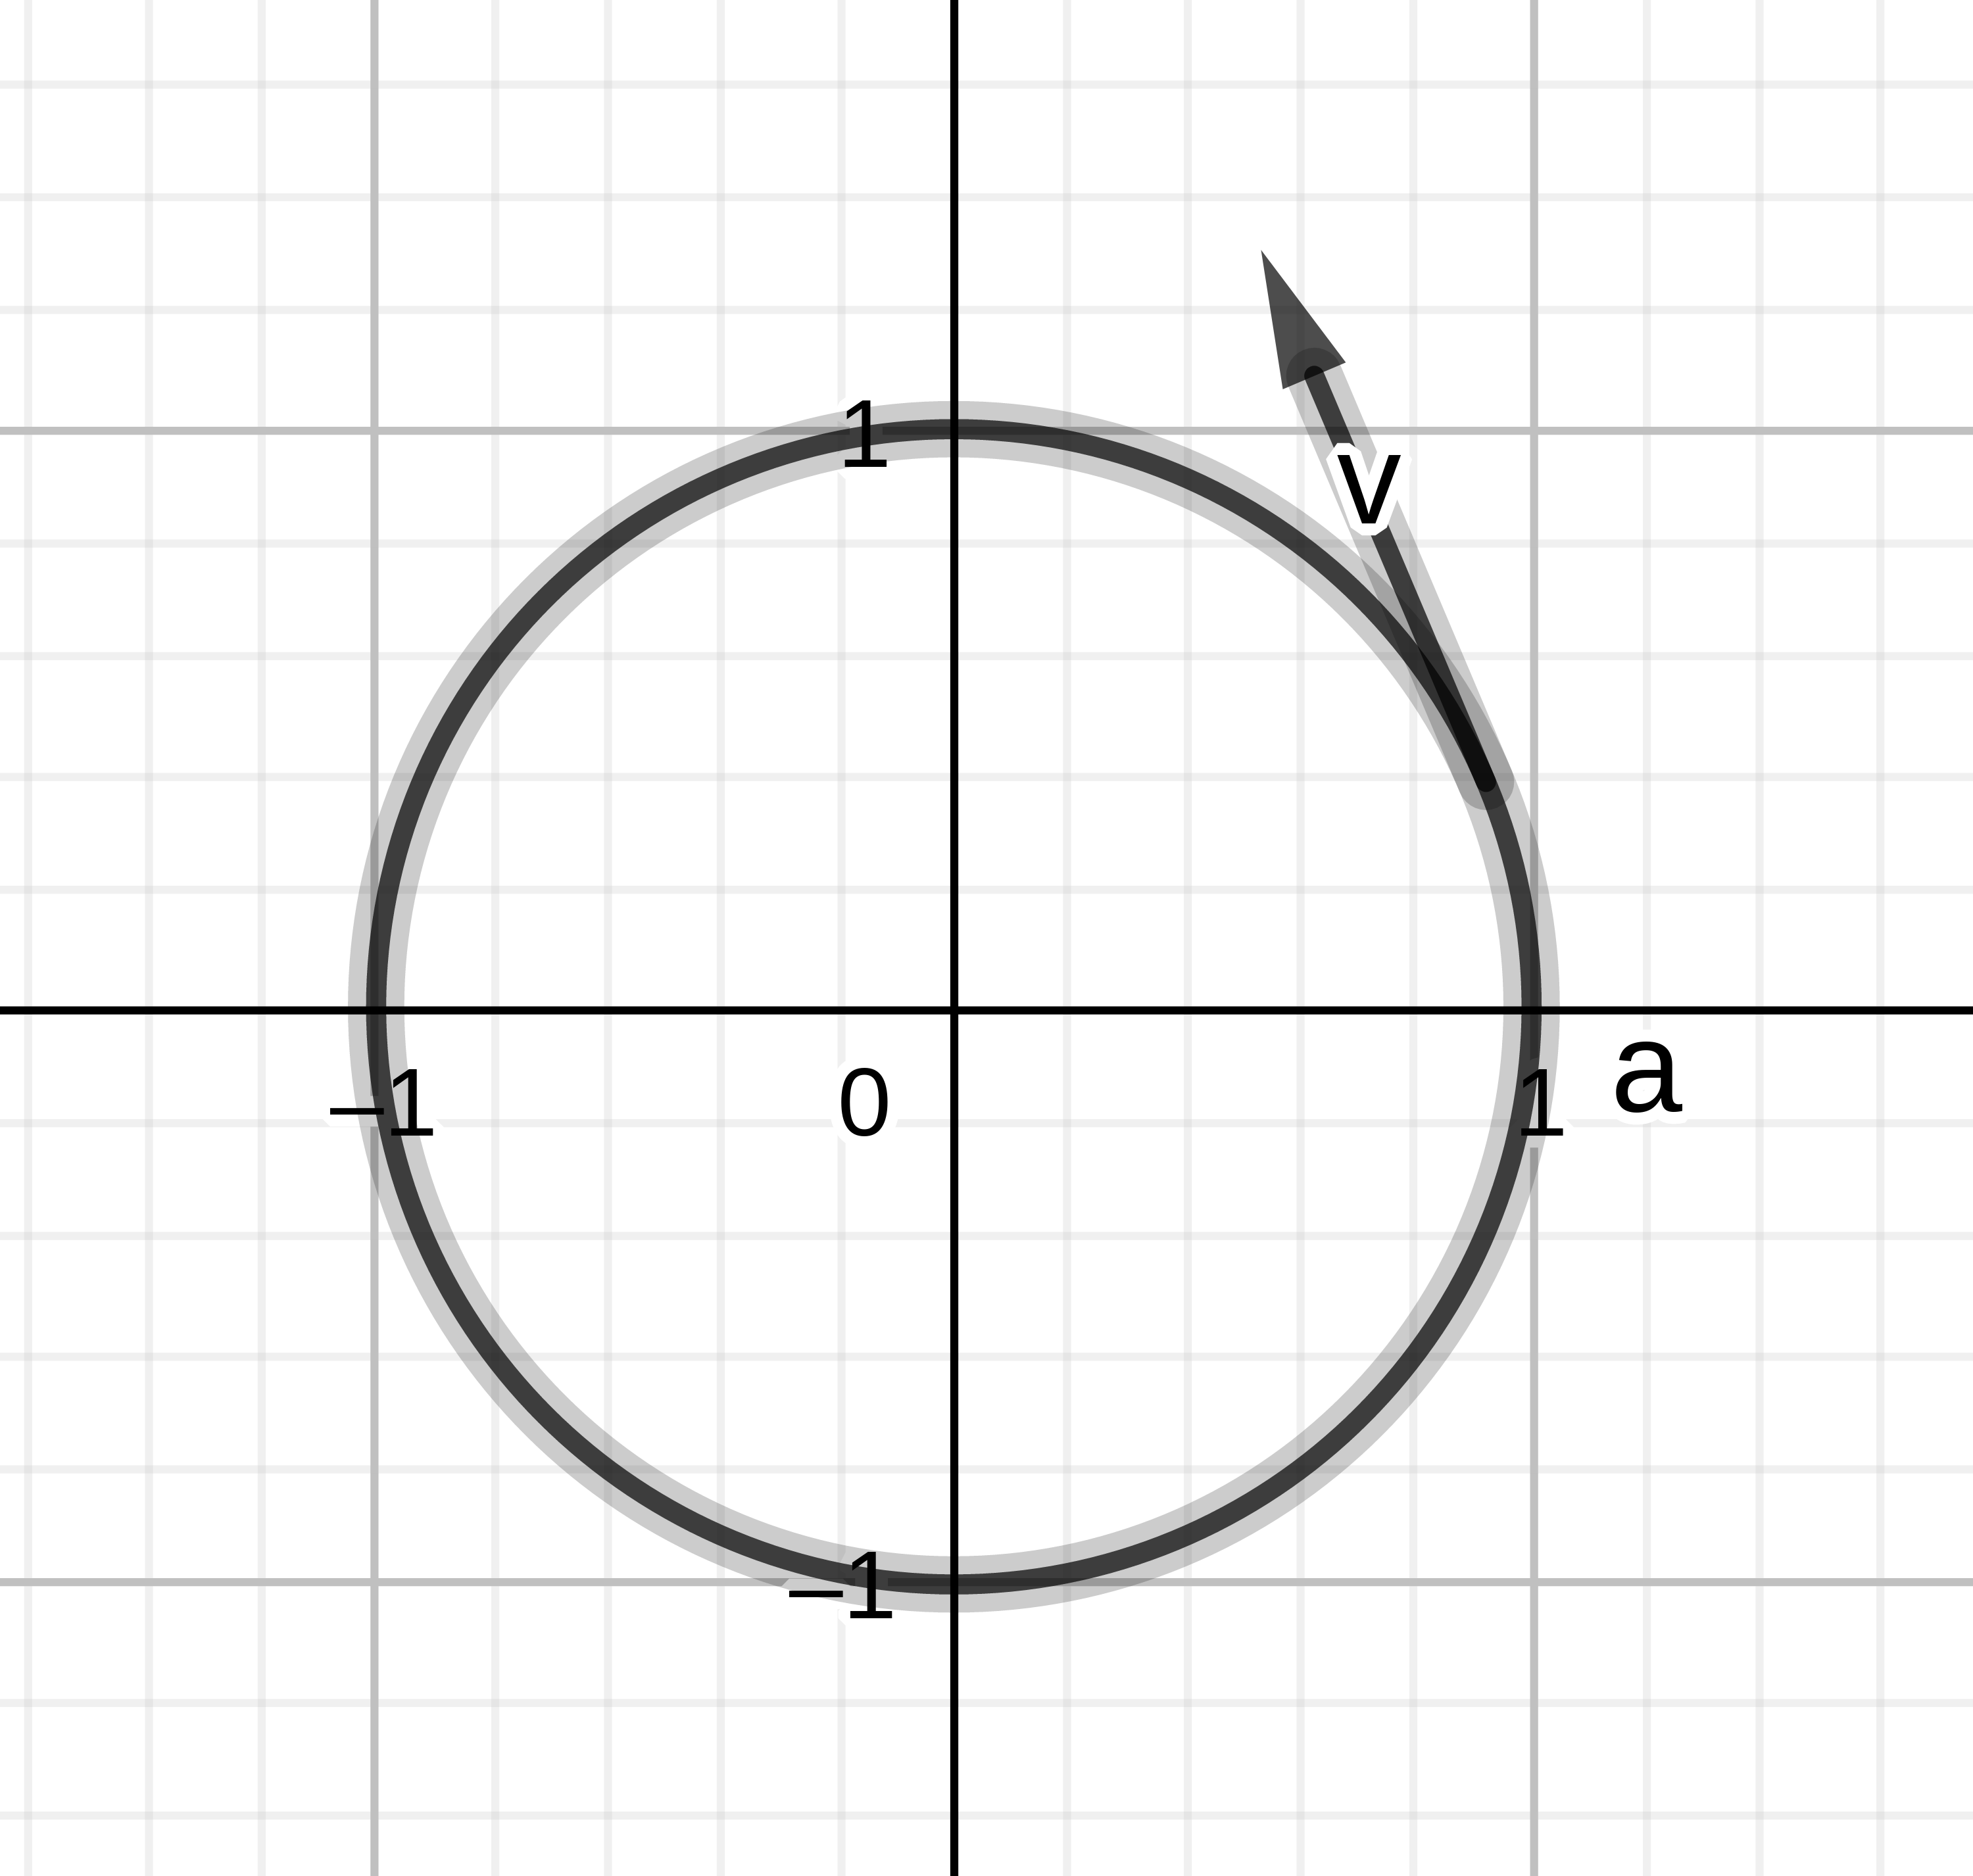
\includegraphics[scale=2]{images/ex1.png}
		\caption{Circunferência uninária e vetor tangente}
	\end{figure}
	
	\item A \emph{limaçon} (ou caracol de Pascal) é a curva parametrizada 
	
	$$\gamma (t) = ((1 + 2\cos (t))\cdot \cos (t); (1 + 2\cos (t))\cdot \sin (t)); t \in \mathbb{R}$$
	
	Faça o desenho desta curva. Observe que o ponto $(0, 0)$ pertence ao traço da curva, e ache o vetor tangente nesse ponto.
	\subitem \textbf{Solução:} O vetor tangente (unitário) é 
	
	\begin{align}
		\vec v(t)&= \dfrac{\gamma'(t)}{||\gamma'(t)||}\nonumber\\
				&= \dfrac{(-\sin (t) (4 \cos t + 1), 2\cos(2t) + \cos t )}{\sqrt{4\cos t+5}}\label{tg2}
	\end{align}
	
	É fácil ver que o ponto $(0,0)$, pois $\gamma(2\pi/3)=\gamma(4\pi/3)=(0,0)$ já que $\cos(2\pi/3)=\cos(4\pi/3)=-1/2$, o que anula $(1+2\cos t)$ que por sua vez anula o vetor $\gamma$. De fato, a Figura \ref{ex2} mostra que a origem é cruzada duas vezes pelo traço.
	
	\begin{figure}[!htb]
		\centering
		\label{ex2}
		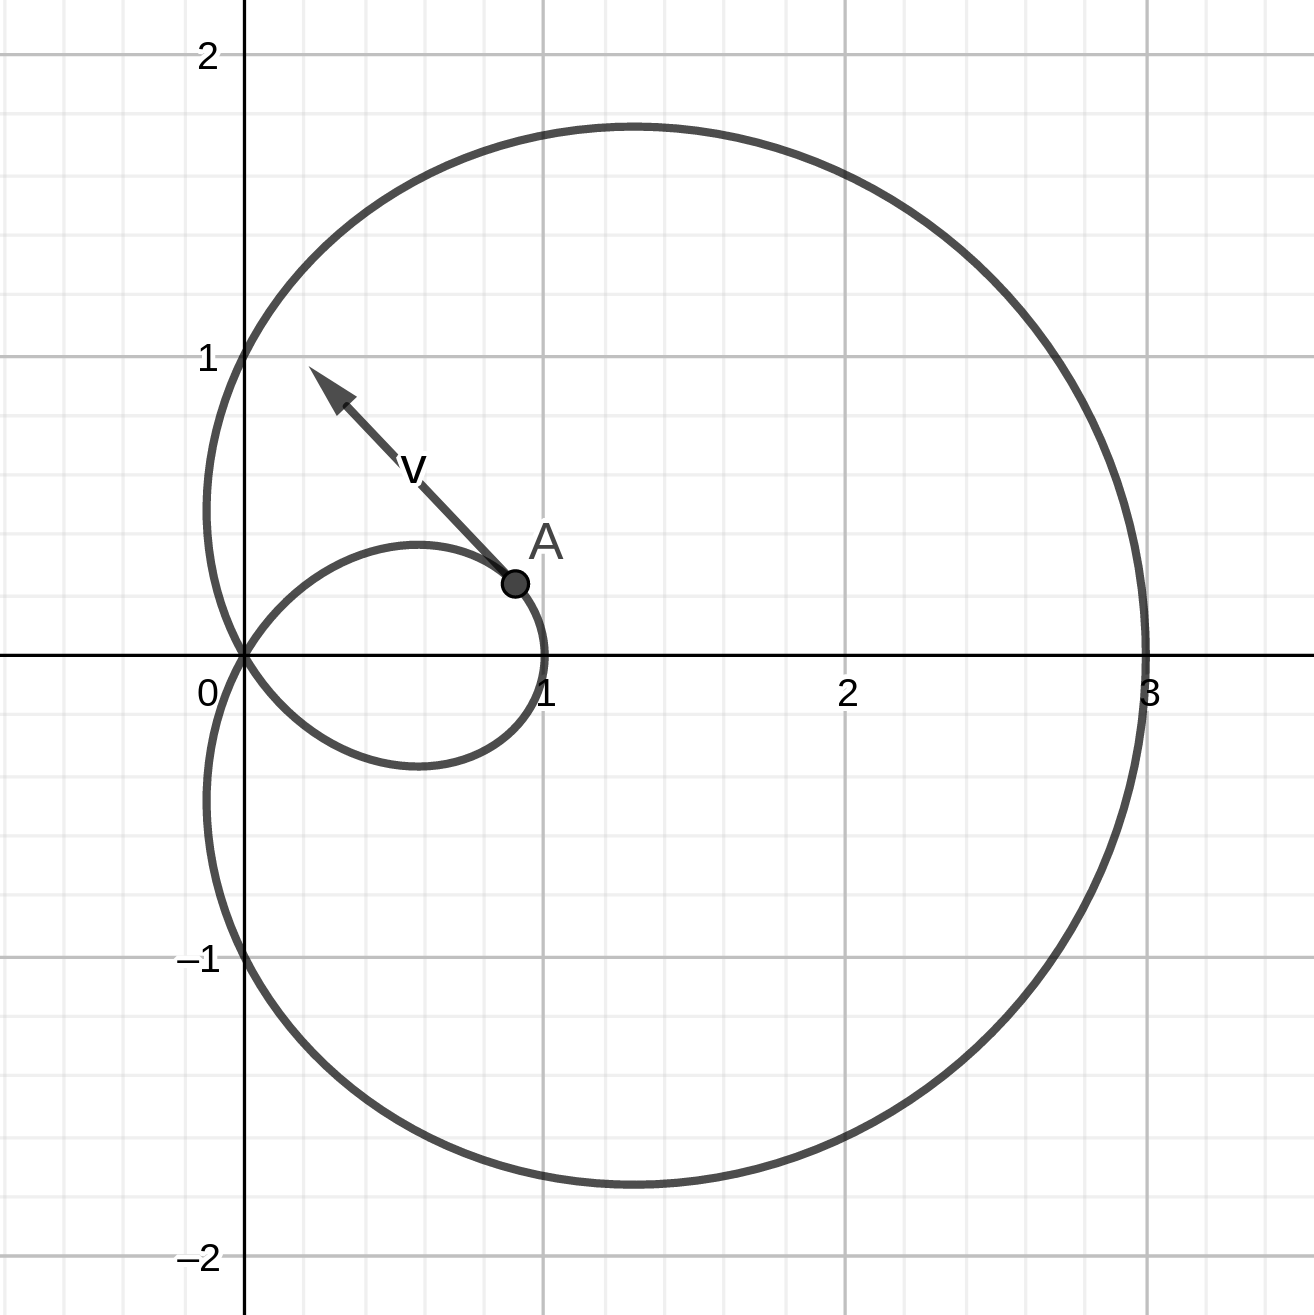
\includegraphics[scale=0.2]{images/ex2.png}
		\caption{Caracol de Pascal e vetor tangente}
	\end{figure}
	De \ref{tg2}, temos que o vetor tangente na origem será:
	

		$v\left(\dfrac{2\pi}3\right)=\left(\dfrac12,-\dfrac{\sqrt3}2\right)$ no primeiro cruzamento e
		
		$v\left(\dfrac{4\pi}3\right)=\left(-\dfrac12,-\dfrac{\sqrt3}2\right)$ no segundo cruzamento.
		
	\item A \emph{Cissoide de Diocles} é a curva definida implicitamente pela equação $$x^3 + xy^2 - 2a^2y^2 = 0$$. Encontre uma parametrização para esta curva. Faça o desenho em Geogebra, incluindo a animação do vetor tangente percorrendo a curva. Busque informação para	entender qual o fenômeno modelado por esta curva que a tornou famosa. (Dica: use $y = xt$ para encontrar uma parametrização da curva).
	
	\subitem \textbf{Solução:} Usando $y=xt$, temos:
	
	\begin{align*}
		x^3+x^3t^2-2ax^2t^2=0\Rightarrow\\
		x^3(1+t^2)=2ax^2t^2
	\end{align*}

	Dado que $1+t^2>0~\forall t \in \mathbb{R}$. A solução considerando $x(t)\neq0$ é:
	
	$x(t)=\dfrac{2at^2}{1+t^2}$ e consequentemente $y(t)=\dfrac{2at^3}{1+t^2}$
	
	Daí vemos que $x=0$ se, e somente se $t=0$ ou $a=0$. E $x<0\leftrightarrow a<0$. Tornando a fórmula consistente.
	
	O vetor tangete (unitário) de $\gamma(t)=(x(t),y(t))$ é
	
	\begin{align*}
	\vec v (t)&= \dfrac{1}{||\gamma'(t)||}(x'(t),y'(t))\\
	&=\dfrac{1 + t^2}{2 |at|\sqrt{4 + t^2} }\left(\dfrac{4 a t}{(1 + t^2)^2},\dfrac{2 a t^2 (t^2 + 3)}{(1+t^2)^2}\right)\\
	&=\left(\dfrac{2\operatorname{sign}(at)}{(1+t^2)\sqrt{4+t^2}},\dfrac{\operatorname{sign}(at)(t^3+3t)}{(1+t^2)\sqrt{4+t^2}}\right)\\
	&=\dfrac{\operatorname{sign}(at)}{(1+t^2)\sqrt{4+t^2}}\left(2,t^3+3t\right)
	\end{align*}
	
	Veja um corte da animação em \href{https://gvmail-my.sharepoint.com/:f:/g/personal/b39398_fgv_edu_br/Euu4MOsNJNNEs3nZTImei1MBK16JRBHHiWUX9SxQeItAEg}{ex3.ggb} na Figura \ref{ex3}
	
	\begin{figure}[!htb]
		\centering
		\label{ex3}
		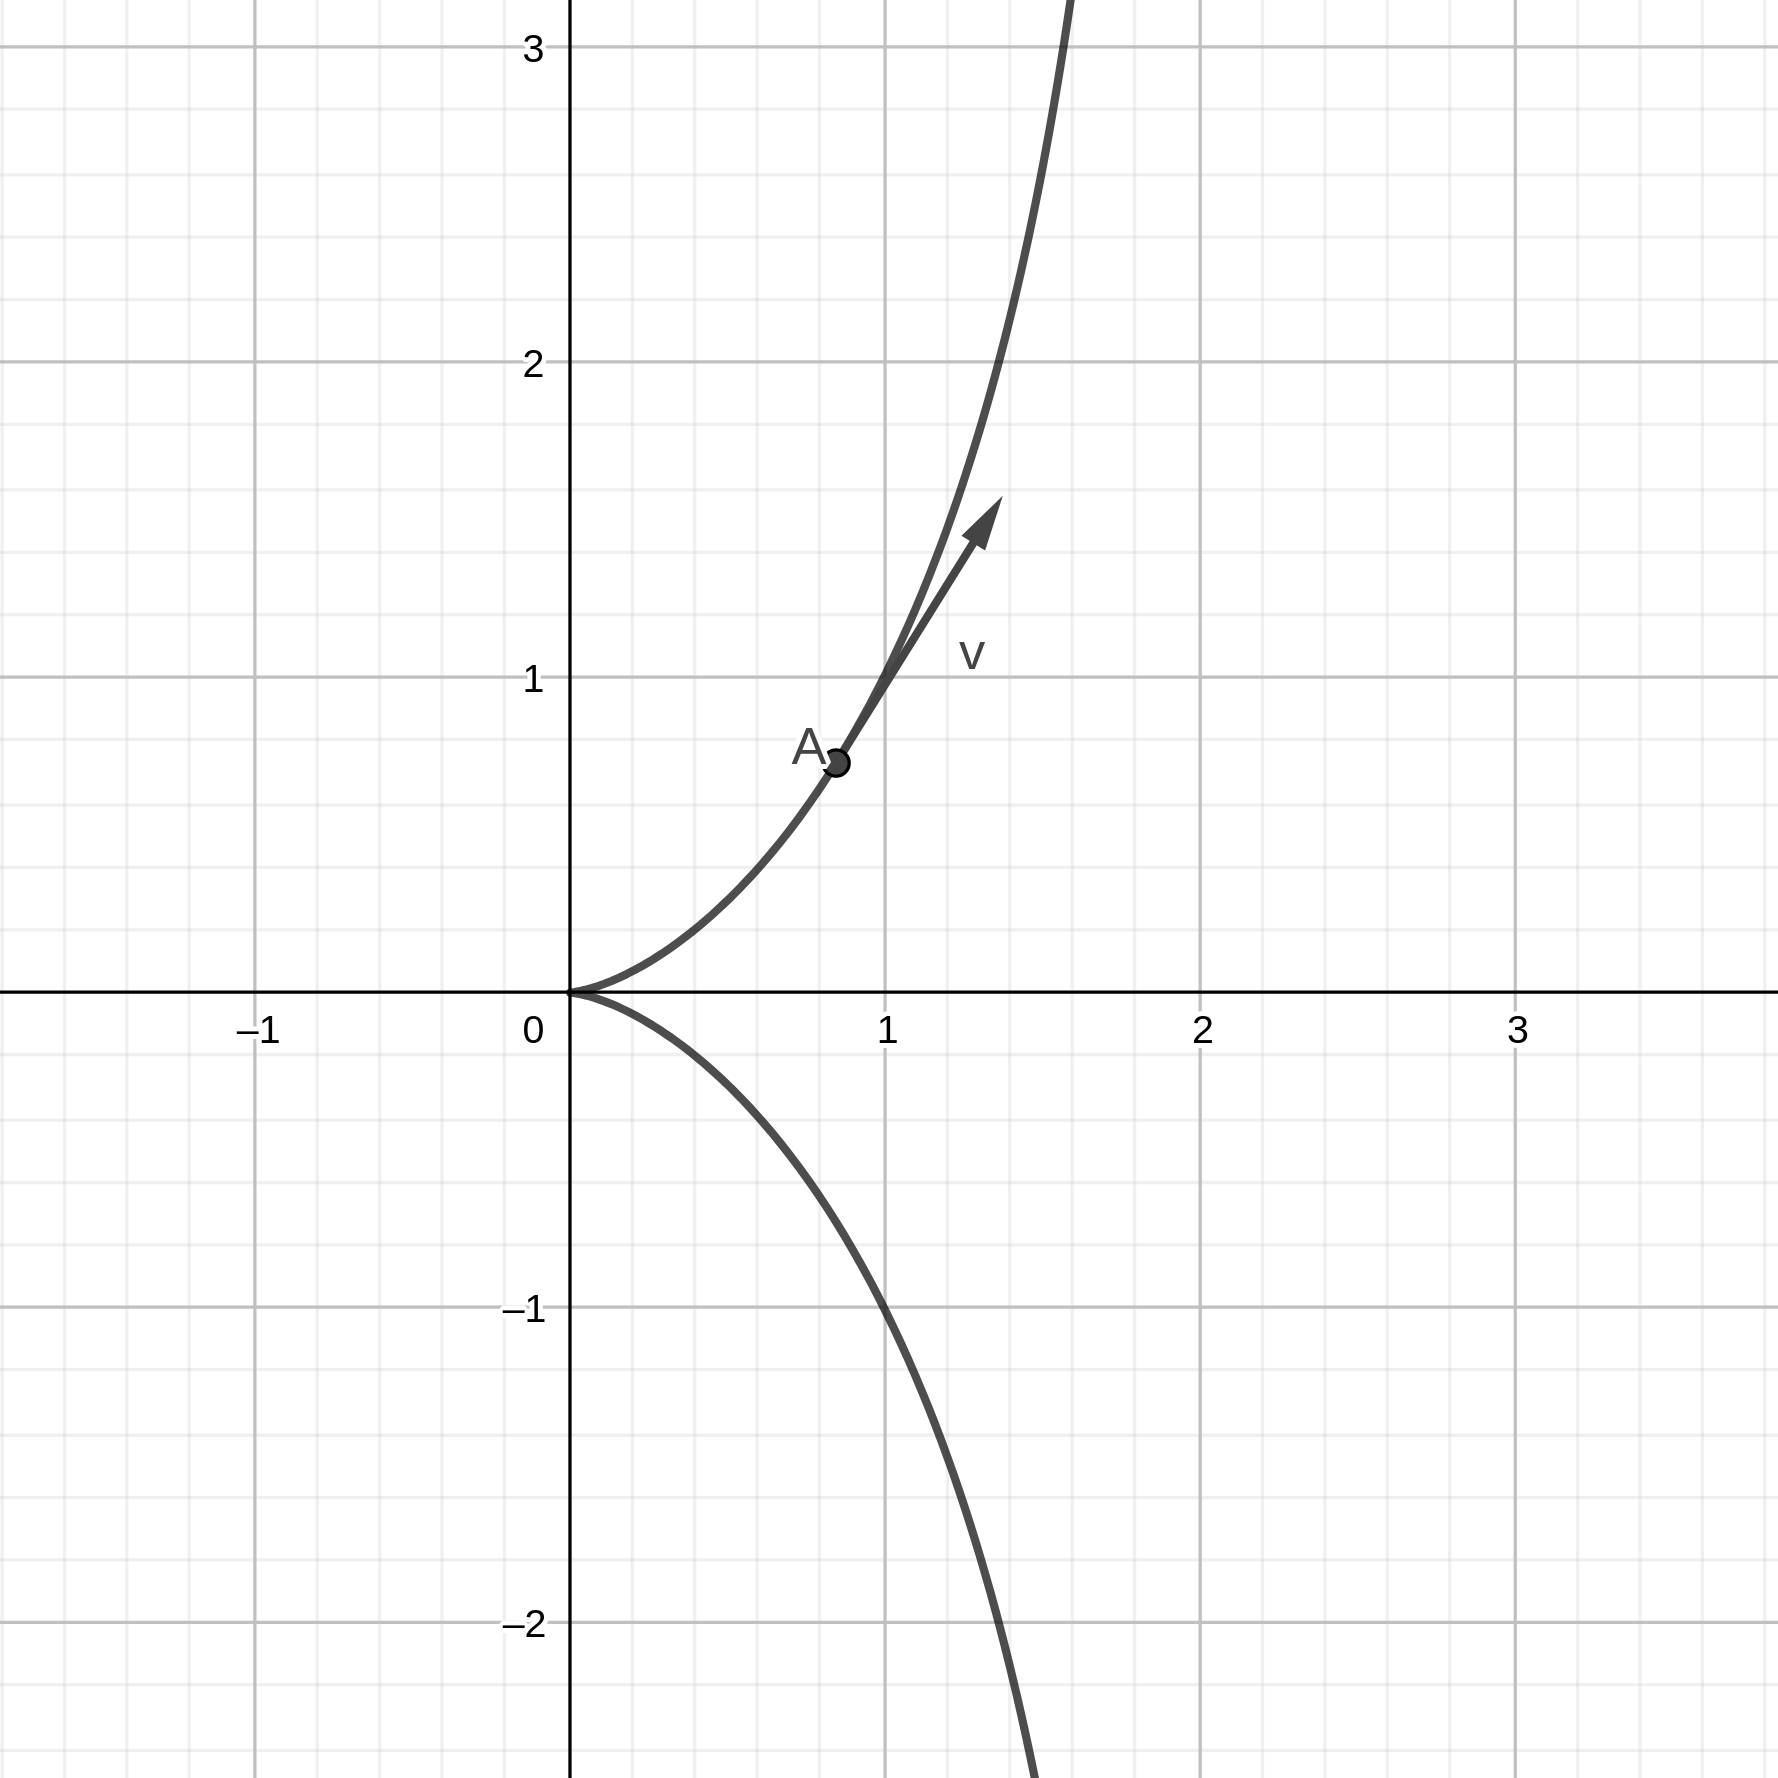
\includegraphics[scale=0.15]{images/ex3.png}
		\caption{Cissoide de Diocles}
	\end{figure}
	
	O curva surgiu do problema resolvido pelo grego Diocles para encontrar médias proporcionais\cite{wiki:Cissoid_of_Diocles}, isto é, dados $a$ e $b$, a curva pode ser usada para encontrar $u$ e $v$ tal que $\dfrac a u =\dfrac u v = \dfrac v b$. Um problema particular, é o problema de Delian: Quanto a medida do lado de um cubo deve aumentar, para que seu volume dobre?
	
	\item O \emph{Folium de Descartes} é definido implicitamenete pela equação]
	$$
	x^3 + y^3 = 3xy$$. 
	
	Encontre uma parametrização para esta curva. Faça o desenho em Geogebra, incluindo a animação do vetor tangente percorrendo a curva. A descrição implicita desta
	curva da origem a uma familia de curvas da forma
	$$F_{\varepsilon}(x, y) = x^3 + y^3 - 3xy - \varepsilon$$.
	
	Observe, usando o Geogebra, a mudança no traço da curva ao mudar de elemento da família (ex.: $\varepsilon=-\frac{1}{10}$).
	
	\subitem \textbf{Solução:} Fazendo $y=x^2t$, temos que a curva será, sobre hipótese $t\neq0$ e $x\neq0$:
	
	$$\gamma(t)=\left(\dfrac{(3t-1)^{1/3}}{t},\dfrac{(3t-1)^{2/3}}{t}\right)$$
	
	O ponto $(0,0)$ é atingido uma vez quando $t=1/3$, mas para fechar a curva implícita, ele não é atingido novamente.
	
	Note que $\displaystyle\lim_{t\to\infty}\gamma(t)=\lim_{t\to\-\infty}\gamma(t)=0$, pois a derivada dos numeradores tende pra $0$ ao $|t|\to\infty$, ou seja, o numerador estabiliza enquanto o denominador só cresce constantemente.
	
	Ao variar o $\varepsilon$ para algo negativo, a curva se subdivide em duas curvas desconexas, ao passo de que a variação positiva faz uma curva regular.
	
	O vetor tangente unitário é:
	
	\begin{align*}
	\vec v (t)&=\dfrac{\gamma'(t)}{||\gamma'(t)||}\\
	&=\dfrac{1}{||\gamma'(t)||}= \left(\dfrac{1 - 2 t}{t^2 (3t-1)^{2/3}}, \dfrac{1 - t}{t^2 (3t-1)^{1/3}}\right)\\
	&=\dfrac{t^2 |3t-1|^{2/3}}{\sqrt{(t - 1)^2 (3t-1)^{2/3} + (1 - 2 t)^2}}\cdot\left(\dfrac{1 - 2 t}{t^2 |3t-1|^{2/3}}, \dfrac{1 - t}{t^2 (3t-1)^{1/3}}\right)\\
	&=\dfrac{\operatorname{sign}((3t-1)^{2/3})}{\sqrt{(t - 1)^2 |3t-1|^{2/3} + (1 - 2 t)^2}}\cdot\left(1 - 2 t, (1 - t)(3t-1)^{1/3}\right)
	\end{align*} 
	
	Veja um corte da animação do vetor tangente em \href{https://gvmail-my.sharepoint.com/:f:/g/personal/b39398_fgv_edu_br/Euu4MOsNJNNEs3nZTImei1MBK16JRBHHiWUX9SxQeItAEg}{ex4.ggb} na Figura \ref{ex4}.
	
	\begin{figure}[!htb]
		\centering
		\label{ex4}
		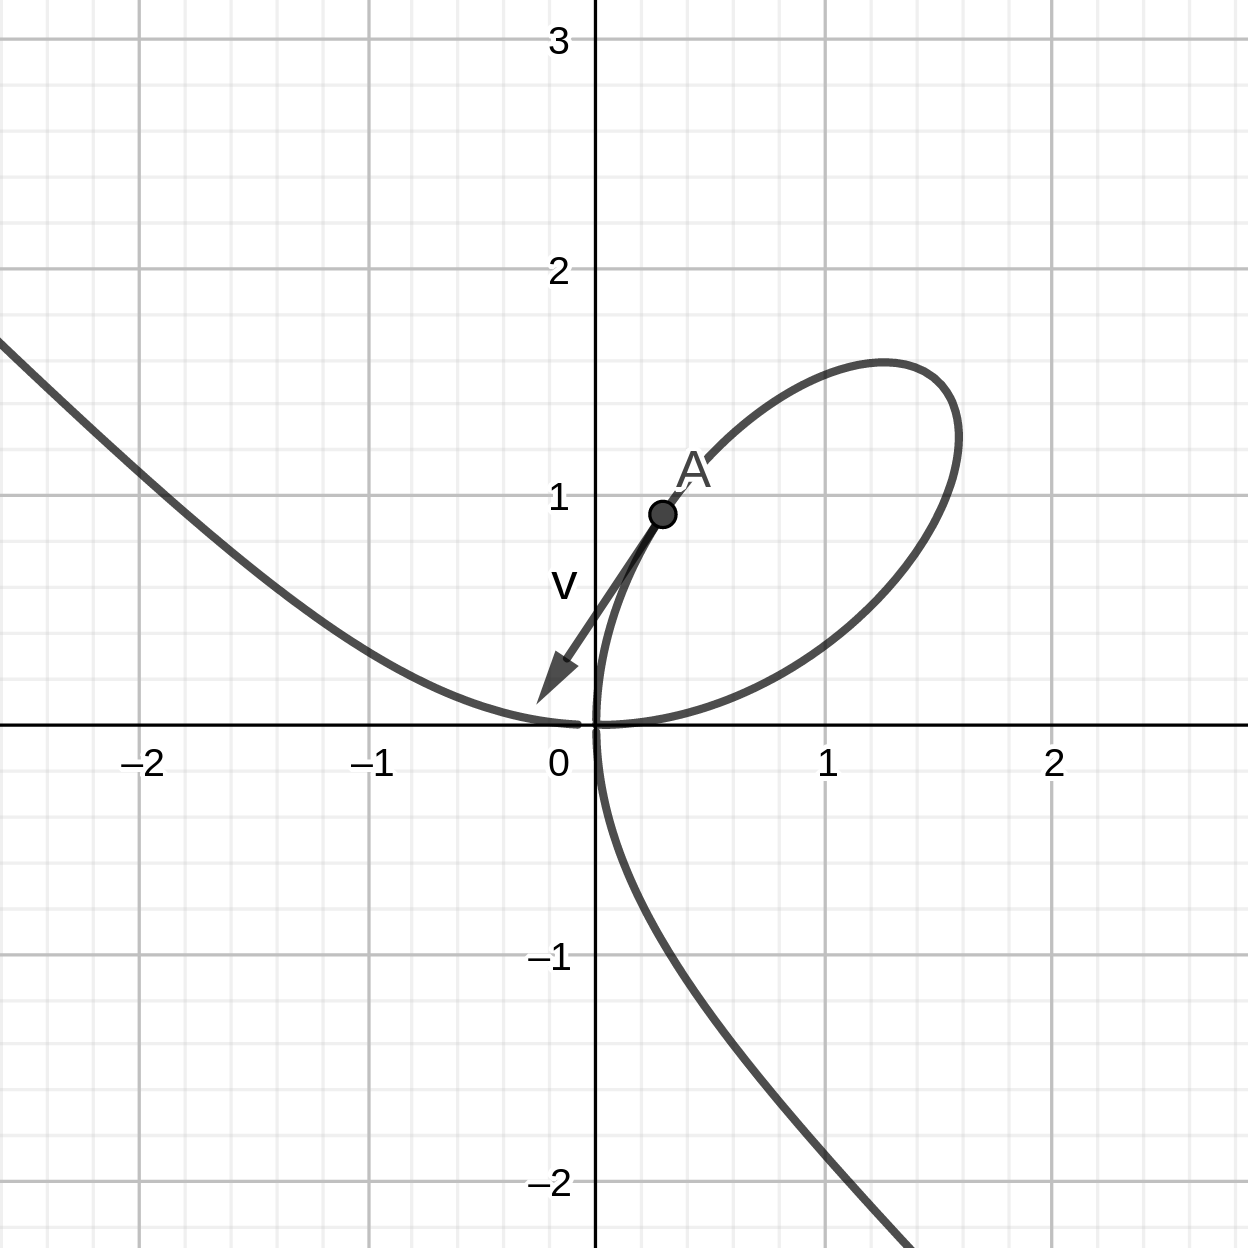
\includegraphics[scale=0.25]{images/ex4.png}
		\caption{Folium de Decartes}
	\end{figure}

	\item Verifique que a aplicação $\alpha(t) = (a \cos(t), b\sin(t)), t \in \mathbb{R}$, com $a$ e $b$ constantes não-nulas, é uma curva parametrizada diferenciável. Descreva o traço de $\alpha$.
	
	\subitem \textbf{Solução:} Temos que provar que $\alpha(t)$ é da classe $C^{\infty}$ \cite{ronaldo}, ou seja, que as derivadas de todas as ordens são contínuas e deriváveis.
	
	Sendo $a,b>0$, temos:
	\begin{align*}
		\alpha'(t)&=(-a\sin t,b \cos t)\\
		\alpha''(t)&=(-a\cos t,-b\sin t)\\
		\alpha^{(3)}(t)&=(a\sin t,-b\cos t)\\
		\alpha^{(4)}(t)&=(a\cos t,b\sin t)\\
	\end{align*}
	
	Veja que após quatro iterações de derivação, voltamos a $\alpha(t)$ original. Como as funções seno e cosseno são deriváveis e contínuas nos reais, e as derivadas de qualquer ordem de $\alpha$ são senos e cossenos, à menos de constantes não-nulas, concluímos que todas as derivadas de $\alpha$ também são deriváveis e contínuas.
	
	Podemos entender o traço da curva olhando pata os pontos notáveis $t=0$, $t=\pi/2$, $t=\pi$ e $t=3\pi/2$.
	
	\begin{align*}
	\alpha(0)&=(a,0)\\
	\alpha(\pi/2)&=(0,b)\\
	\alpha(\pi)&=(-a,0)\\
	\alpha(3\pi/2)&=(0,-b)
	\end{align*}
	
	Esses pontos são estremidades de uma elipse de eixos $2a$ e $2b$, com equação implícita $\dfrac{x^2}{a^2}+\dfrac{y^2}{b^2}=1$.
	\item Obtenha uma curva regular $\alpha: \mathbb{R}\to\mathbb{R}^2$ tal que $\alpha(0) = (2, 0)$ e $\alpha' (t) = (t^2 , e^t)$.
	\subitem \textbf{Solução:}
	Tomemos  $\beta(t)=\displaystyle\int_0^t\alpha'(s)ds$.
	
	\begin{align*}
	\displaystyle\int_0^t\alpha'(s)ds&=\int_0^t(s^2 , e^s)ds\\&=\left.\left(\dfrac{s^3}3,e^s\right)\right|_{s=0}^{s=t}\\
	&=\left(\dfrac{t^3}3,e^t\right)-\left(0,1\right)\\
	&=\left(\dfrac{t^3}3,e^t-1\right)
	\end{align*}
	
	Note que $\beta'(t)=(t^2 , e^t)$, mas $\beta(0)=(0,0)$. Já que adição de constantes não afeta a derivada, podemos definir $\alpha(t)=\beta(t)+(2,0)=\left(\dfrac{t^3}3+2,e^t-1\right)$ e cumpriremos as exigências.
	
	\item Seja $\alpha : I \to \mathbb{R}^2$ uma curva regular. Prove que $||\alpha'(t)||$ á constante se, e somente se,
	para cada $t \in I$, o vetor $\alpha'' (t)$ é ortogonal a $\alpha'(t)$.
	\subitem \textbf{Solução:} ($\Longrightarrow$) Dado $\alpha(t)$, se $||\alpha'(t)||$ é constante queremos provar que $\alpha' (t)\perp\alpha'' (t)$ para todo $t\in I$.
	
	É fácil ver que $||\alpha'(t)||=c\Rightarrow||\alpha'(t)||^2=c^2$, com $c\in\mathbb{R}$, ou seja se a norma da derivada é constante, o quadrado da norma também é. Já que $||\alpha'(t)||^2=\langle\alpha'(t),\alpha'(t)\rangle$, temos que, $||\alpha'||=c$ implica em :
	
	\begin{align*}
		&~\langle\alpha',\alpha'\rangle=c^2\\\Rightarrow&~
		\dfrac{d}{dt}\langle\alpha',\alpha'\rangle=0\\\Rightarrow&~
		\langle\alpha'',\alpha'\rangle+\langle\alpha'',\alpha'\rangle=0\\\Rightarrow&~
		2\langle\alpha'',\alpha'\rangle=0\\\Rightarrow&~
		\langle\alpha'',\alpha'\rangle=0
	\end{align*}
	
	O parâmetro $t$ foi omitido, mas a conclusão acima implica que 
	
	$$\forall ~t \in I~\alpha' (t)\perp\alpha'' (t)$$
	
	($\Longleftarrow$) A recíproca é facilmente verificácel pois todos as implicações acima são invertíveis. Assim, se $\alpha'\perp\alpha''$, o produto escalar será nulo, implicando pela regra do produto usada de forma inversa, que a derivada de  $\langle\alpha',\alpha'\rangle$ é nula, o que mostra que tal produto é constante, implicando finalmente que $||\alpha'(t)||=\sqrt{\langle\alpha',\alpha'\rangle}$ é constante. 
	\begin{flushright}
		\textbf{Q.E.D}
	\end{flushright}

	\item Prove que, se uma curva regular $\alpha(t) = (x(t), y(t)), t \in I \subset \mathbb{R}$, é tal que $x'(t) \neq  0~\forall t \in I$,	então o traço de $\alpha$ é o gráfico de uma função diferenciável.
	\subitem \textbf{Solução:}
	
	Sejam $X=\{x(t);t \in  I\}$ e $Y=\{y(t);t\in I \}$ e $\alpha(I)$ o traço da curva.
	
	\begin{align*}
		f: X &\to Y\\
		x&\mapsto f(x)=y\text{ tal que }(x,y)\in\alpha(I)
	\end{align*}
	
	Vamos provar for absurdo que $f$ é uma função bem definida.
	
	Suponha então por contradição, que $\exists~x^*\in X$ tal que $f(x^*)$ mapeia mais de 1 valor em $Y$, isto é, $\exists~y_1,y_2\in Y$, com $y_1\neq y_2$ tal que $f(x^*)=y_1$ e $f(x^*)=y_2$
	
	Tome $t_1=\alpha^{-1}(x^*,y_1)$ e $t_2=\alpha^{-1}(x^*,y_2)$, e façamos a restrição da componente $x(t)$ de $\alpha$ para o intervalo $I^*=[t_1,t_2]$ supondo, sem perda de generalidade, que $t_1<t_2$; tal restrição está bem definida, pela boa definição das componentes de $\alpha$.
	
	
	\textbf{Teorema de Rolle}\cite{lima1981curso}. Seja $g:[a,b]\to\mathbb{R}$ contínua, tal que $g(a)=g(b)$. Se $g$ é derivável em $(a,b)$ então existe um ponto $c\in(a,b)$ onde $g'(c)=0$.
	
	Como $x(t)$ é contínua e derivável para todo $t$ em $I$, vale que $x:I^*\to\mathbb{R}$ é contínua e derivável. Note que $x(t_1)=x(t_2)=x^*$. Pelo teorema acima, $\exists ~t^*\in(t_1,t_2)$ tal que $x'(t^*)=0$, \textbf{absurdo, pela hipótese de regularidade}.
	
	Logo $f$ está bem definida.
	
	Para provar a diferenciabilidade, precisamos provar que $f'(x)$ existe para todo ponto em $X$, ou seja, $\lim_{x\to a}\dfrac{f(x)-f(a)}{x-a}$ existe $\forall a \in X$.
	
	Sejam $s_1,s_2\in I$ tais que $x(s_1)=x$ e $x(s_2)=a$ assim,
	
	\begin{align*}&~~~~~\lim_{x\to a}\dfrac{f(x)-f(a)}{x-a}\\&=\lim_{x(s_1)\to x(s_2)}\dfrac{f(x(s_1))-f(x(s_2))}{x(s_1)-x(s_2)}\\&=\lim_{s_1\to s_2}\dfrac{y(s_1)-y(s_2)}{x(s_1)-x(s_2)}\end{align*}
	
	A última igualdade vale pois, pela continuidade de $x(t)$, podemos trocar o limite $x(s_1)\to x(s_2)$ para $s_1\to s_2$; e pela boa definição de $f$, $f(x(s_1))-f(x(s_2))=y(s_1)-y_(s_2)$.
	
	Podemos usar o fato de que, dentro do limite, $s_1\neq s_2$, e dividir numerador e denominador por $s_1-s_2$. Assim,
	
	$$\lim_{s_1\to s_2}\dfrac{y(s_1)-y(s_2)}{x(s_1)-x(s_2)}=\lim_{s_1\to s_2}\dfrac{~\frac{y(s_1)-y(s_2)}{s_1-s_2}~}{~\frac{x(s_1)-x(s_2)}{s_1-s_2}~}$$
	
	Veja que $\displaystyle\lim_{s_1\to s_2}\dfrac{x(s_1)-x(s_2)}{s_1-s_2}$ é a definição de $\dfrac{d}{dt}x(t)$, que por hipótese é não-nula para todo $t\in I$. O limite do quociente acima será então o quociente do limite, que pela definição de derivada é igual a $\dfrac{~\frac{d}{dt}y(t)~}{~\frac{d}{dt}x(t)~}$, fração que está bem definida para todo $t\in I$. Portanto, prova-se que $\dfrac{d}{dx}f(x)$ existe para todo $x\in X$.
	
	\begin{flushright}
		\textbf{Q.E.D}
	\end{flushright}
	\item Considere a espiral logaritmica $\gamma : \mathbb{R} \to \mathbb{R}^2$ definida por $$\gamma(t) = (e^t \cdot \cos(t),e^t\cdot \sin(t))$$.	Desenhe a curva em ambiente computacional e mostre que o ângulo entre $\gamma(t)$ e o vetor
	tangente em $\gamma(t)$ não depende de $t$.
	
	\subitem \textbf{Solução:}
	
	Veja um corte da animação do vetor tangente em \href{https://gvmail-my.sharepoint.com/:f:/g/personal/b39398_fgv_edu_br/Euu4MOsNJNNEs3nZTImei1MBK16JRBHHiWUX9SxQeItAEg}{ex9.ggb} na Figura \ref{ex9}.
	
	\begin{figure}[!htb]
		\centering
		\label{ex9}
		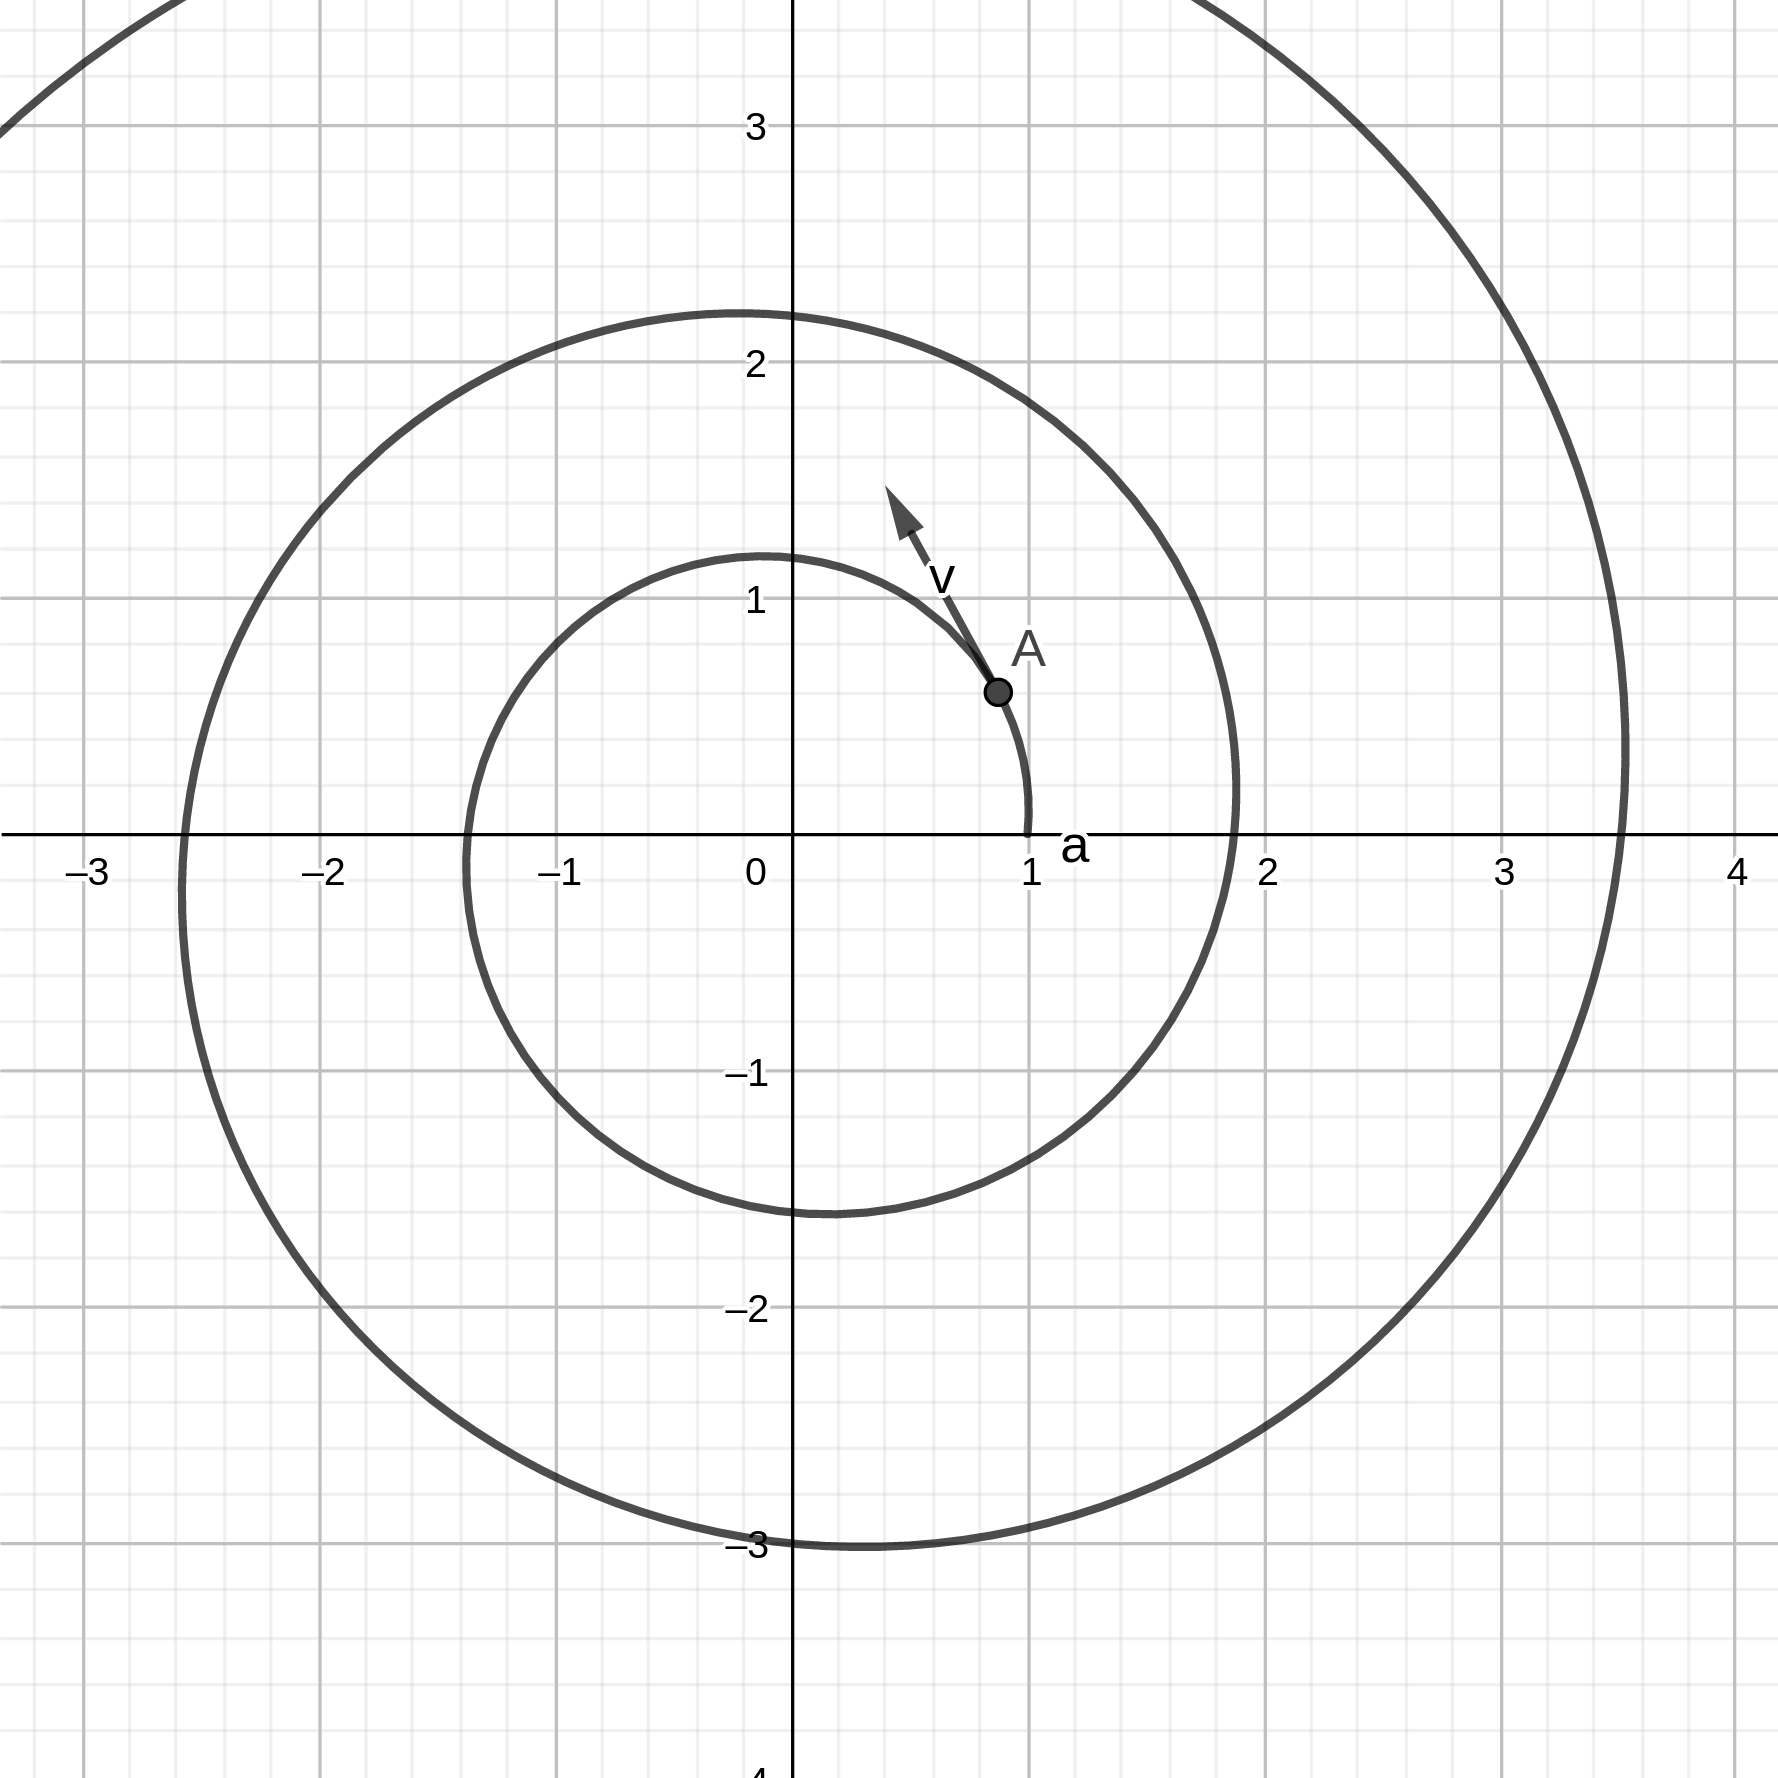
\includegraphics[scale=0.2]{images/ex9.png}
		\caption{Espiral logarítmica}
	\end{figure}

	De fato, ao executar a animação, o ângulo entre o vetor tangente e a curva não muda. Seja $\theta_t$ o ângulo para dado $t$ entre o vetor tangente o o eixo x do plano. Se o vetor tangente $\vec v(t)$ é unitário e centrado na origem, então seu ponto final coincide com $(\cos \theta _t,\sin\theta _t)$.
	
	Calculando v, temos:
	%{(k cos(t) - sin(t))/sqrt(k^2 + 1), (k sin(t) + cos(t))/sqrt(k^2 + 1)}
	\begin{align*}
		\vec v (t)&=\dfrac{1}{||\gamma'(t)||}\left(e^{k t} (k \cos(t) - \sin(t)), e^{kt} (k \sin(t) + \cos(t))\right)\\
		&=\dfrac{e^{kt}}{e^{k t}\sqrt{k^2 + 1} }\left(k \cos(t) - \sin(t), k \sin(t) + \cos(t)\right)\\
		&=\dfrac{1}{\sqrt{k^2 + 1} }\left(k \cos(t) - \sin(t), k \sin(t) + \cos(t)\right)
	\end{align*}
	
	Assim, à menos de translaçoes por múltiplos de $2\pi$ temos:
	
	\begin{align*}
	\sin (\theta_t)&=\dfrac{k \sin(t) + \cos(t)}{\sqrt{k^2 + 1}}\\
	\cos(\theta_t)&=\dfrac{k \cos(t) - \sin(t)}{\sqrt{k^2 + 1} }
	\end{align*}
	
	Ou seja, $\tan(\theta_t)=\dfrac{k \sin(t) + \cos(t)}{k \cos(t) - \sin(t)}=\dfrac{k\tan t+1}{k-\tan t}=\dfrac{\tan t+\frac1 k}{1-\frac1 k\tan t}$, considerando $t$ tal que o cosseno esteja definido.
	
	Usando a fórmula, $\arctan a + \arctan b = \arctan \dfrac {a + b} {1 - a b}$, temos que:
	
	$\theta_t=\arctan(\tan \theta_t)=\\\arctan\left(\dfrac{\tan t+\frac1 k}{1-\frac1 k\tan t}\right)=\\\arctan(\tan t)+\arctan(\frac1 k)= \\t+\arctan(\frac1 k)$
	
	Assim $\theta_t=t+\arctan(\frac1 k)$, o ângulo entre $v$ e o eixo x do plano.
	
	Para obter o ângulo entre o vetor e a curva\cite{wiki:Tangential_angle} para $t$ dado, subtrai-se de $\theta_t$ tal parâmetro $t$ e obtemos $\arctan(\frac1 k)$ como um ângulo invariante entre a curva e o vetor.
	
	\begin{flushright}
		\textbf{Q.E.D}
	\end{flushright}
%	\begin{align*}
%	\sin (\theta_t)=\dfrac{k \sin(t) + \cos(t)\right}{\sqrt{k^2 + 1}}%\\
%	%\cos(\theta_t)&=\dfrac{k \cos(t) - \sin(t)}{\sqrt{k^2 + 1} }
%	\end{align*}
%	
\end{enumerate}

	
\newpage

% \addcontentsline{toc}{section}{Referências}
\bibliographystyle{plain}
\bibliography{refs}
\end{document}